\section{Approach} \label{Sec:approach}
%Our main goal in this work is to generate client-side test cases coupled with
%effective test oracles, capable of detecting regression \javascript and DOM-level faults. 
%Further, we aim to achieve this goal as efficiently as possible. Hence, we make two design decisions. First, we assume that there is a finite amount of time available to generate test cases. Consequently we guide the test generation  to maximize coverage under a given time constraint. 
%The second decision is to minimize the number of test cases and oracles generated to only include those that are essential in detecting potential faults. %Thus, we only include useful oracles that help testers to find the fault without the need for checking the whole state of the system. 
%Consequently, to examine the correctness of the test suite generated, the tester would only need to examine a small set of assertions, which minimizes their effort.
%
%Our approach generates test cases and oracles at two complimentary levels:
%\begin{description}[noitemsep, nolistsep]
%\item[DOM-level event-based tests] consist of DOM-level event sequences and assertions to check the application's behaviour from an end-user's perspective. 
%\item[Function-level unit tests]  consist of unit tests with assertions that verify the functionality of \javascript code at the function level.
%\end{description}
%
%An overview of the technique is depicted in \figref{approach-view}. 
%At a high level, our approach is composed of three main steps:
%
%\begin{figure}[!t]
%  \centering
%  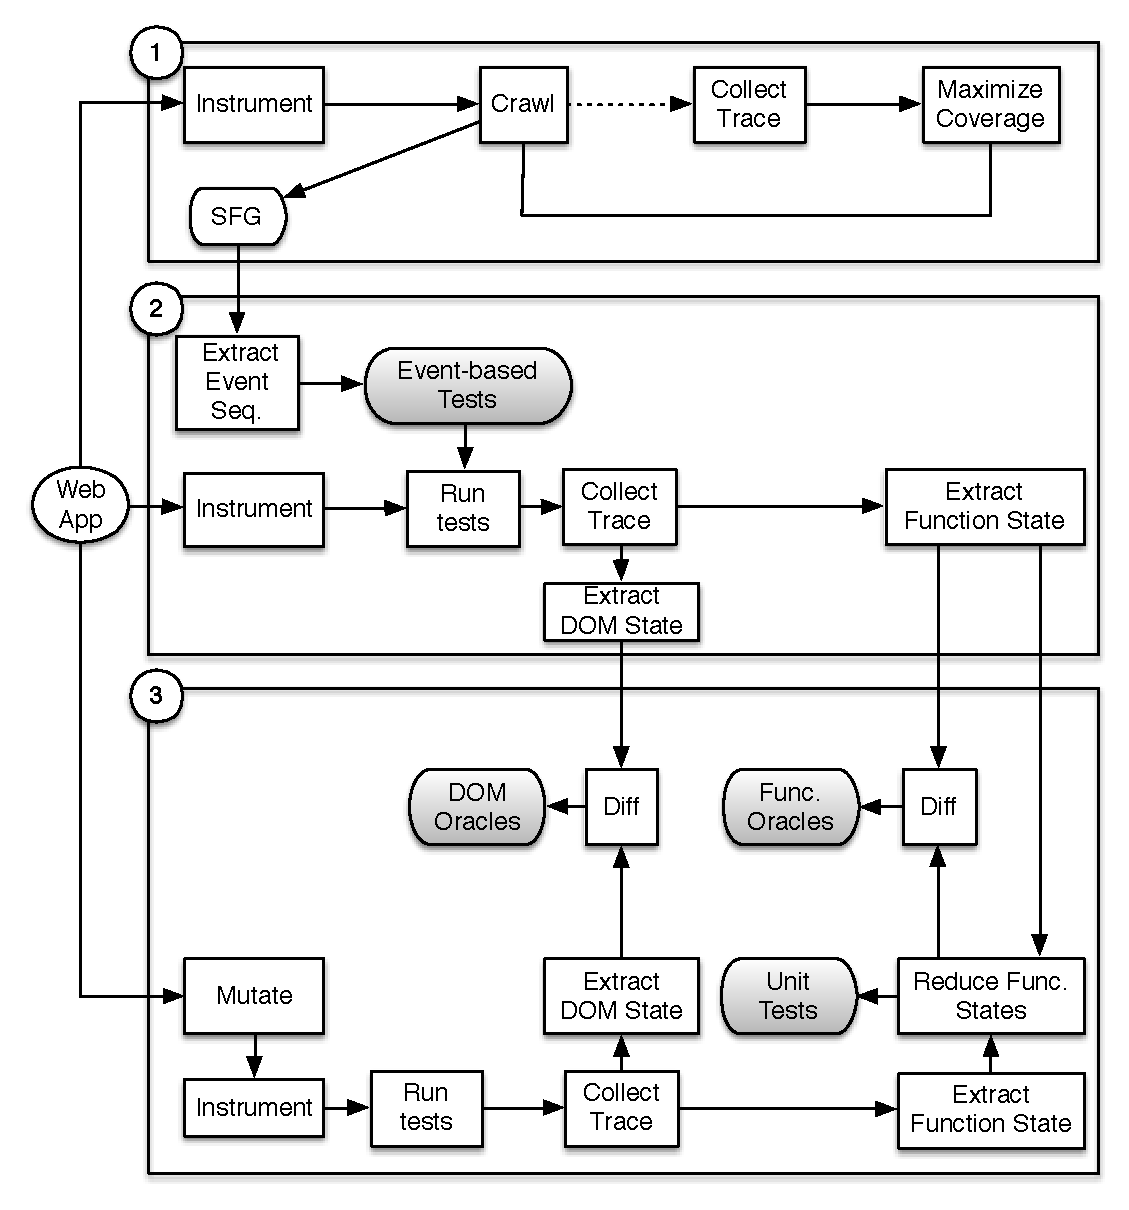
\includegraphics[width=1\hsize]{fig/approach-view-revised}
%  \mycaption{Overview of our test generation approach.}
%  \vspace{-0.1in} 
%  \label{Fig:approach-view}
%\end{figure}
%
%\begin{enumerate}[noitemsep,nolistsep]
% 
%\item In the first step (Section~\ref{Sec:funcCovg}), we dynamically explore various states of a given web 
%application, in such a way as to maximize the number of functions that are covered throughout the program execution. The output of this initial step is a state-flow graph (SFG) \cite{mesbah:tse12}, capturing the explored dynamic DOM states and event-based transitions between them. 
%
%\item In the second step (Section~\ref{Sec:testCaseGen}), %test cases are generated at the DOM event and \javascript function levels. We 
%we use the inferred SFG to generate event-based test cases. %The execution trace is collected through instrumenting the code and then automatically executing the application using the application's state machine obtained from the function exploration phase.
%We run the generated tests against an instrumented version of the application. From the execution trace obtained, we extract DOM element states as well as \javascript function states at the entry and exit points, from which we generate function-level unit tests.
%To reduce the number of generated test cases to only those that are constructive, we devise a \emph{state abstraction} algorithm that minimizes the number of states by selecting representative function states.
%
%\item To create effective test oracles for the two test case levels, we automatically generate mutated versions of the application (Section~\ref{Sec:oracleGen}).
%Assuming that the original version of the application is fault-free, the test oracles are then generated at the DOM and \javascript code levels by comparing the states traced from the original and the mutated versions.
%
%\end{enumerate}
%Next, we describe each of these three steps in detail.

%\subsection{Maximizing Function Coverage} 
\label{Sec:funcCovg}

%\IncMargin{0.5em}
\begin{algorithm}[t]
{\scriptsize
\SetKwInOut{Input}{input}\SetKwInOut{Output}{output}
\Input{A Web application $App$, the maximum exploration time $t$, the maximum number of states to explore $n$}
\Output{The obtained state-flow graph \textit{SFG}}
\BlankLine
\nl \textit{App} $\leftarrow \textsc{Instrument}(App)$ \\
\nl \textit{SFG} $\leftarrow \textsc{AddInitialState}(App)$ \\
\Begin {
\nl \While {$\textsc{ConstraintSatisfied}(t,n)$}{
\nl 	\textit{NES} $\leftarrow \textsc{GetNotExpandedStates}($\textit{SFG}$)$\\
\nl    \textit{Trace} $\leftarrow \textsc{CollectTrace}(App)$ \\
\nl 	\textit{NEF} $\leftarrow \textsc{GetNotVisitedFuncs}(\textit{Trace})$\\
\nl 	\For {$s_i \in$ \textit{NES}}{
\nl			$C_{s_i} \leftarrow \textsc{GetClickables}(s_i)$\\
\nl			$F \leftarrow \textsc{GetUniqFuncHandls}(C_{s_i}, \textit{NEF})$\\
\nl			\For {$f \in$ \textit{F}}{
\nl				$\textit{PotClb} \leftarrow \textsc{GetPotentialClbs}(f, \textit{NEF})$
				}
\nl			$\textit{Score}_{s_i} \leftarrow F + PotClb$	
			}
\nl		$\textit{MaxState} \leftarrow \textsc{GetMaxScoreState}(\textit{Score}_s)$\\			
\nl 	$\textit{UniqFuncHandlsClb} \leftarrow \textsc{GetUniqFuncHandls}(\textit{MaxState})$\\	 	
\nl 	\For {$c \in UnqFuncHandlsClb$}{
\nl			\If { ($\textsc{FireEvent}(c)$) }{
					$state \leftarrow \textsc{GetBrowserState}()$\\
\nl				$\textit{SFG}.\textsc{Update}(state, c)$\\
\nl				\textit{Trace} $\leftarrow \textsc{CollectTrace}(App)$ \\					
\nl				\textit{NEF} $\leftarrow \textsc{GetNotVisitedFuncs}(\textit{Trace})$\\
\nl				$state.\textsc{UpdateClickables}()$\\
				}
			}
		}
\nl return \textit{SFG}
}
\caption{Function Coverage Maximization}
\label{Alg:funcCovgMax}
}
\end{algorithm}
%\DecMargin{lem}
In this step, our goal is to maximize the number of functions that can be covered, while exercising the program's event space. 
To that end, our approach combines static and dynamic analysis to decide which state and event(s) should be selected for expansion to maximize the probability of covering uncovered \javascript functions. While exploring the web application under test, our function coverage maximization algorithm 
%, depicted in \algref{funcCovgMax}, 
selects a next state for exploration, which has the maximum value of the sum of the following two metrics:

\headbf{1. Potential Uncovered Functions}  This pertains to 
the total number of unexecuted functions that can potentially be visited through the execution of DOM events in a given DOM state $s_i$. When a given function $f_i$ is set as the event-handler of a DOM element $d \in s_i$, it makes the element a potential clickable element in $s_i$. This can be achieved through various patterns in web applications depending on which DOM event model level is adopted. To calculate this metric, our algorithm identifies all \javascript functions that are directly or indirectly attached to DOM elements as event handlers, in $s_i$ through code instrumentation and execution trace monitoring.  
%Patterns that our approach currently detects include:
%\begin{itemize}[noitemsep]
%\item Inline in HTML code, e.g., \code{<DIV onclick="foo();">};
%\item DOM Event Level 1, e.g., \code{e.onclick=foo};
%\item DOM Event Level 2 \cite{w3c-event2}, e.g., \code{e.addEventListener(\-type, foo)};
%\item jQuery binding \cite{jquery-api}, e.g., \code{e.click(foo)}, \code{e.on(`click', foo)}, \code{e.bind(`click', foo)}. 
%\end{itemize}
%
%Unbinding elements is also detected through the following two patterns: (1) \code{e.removeEventListener(type, foo)}, and \code{e.un\-bind(type)}.

%Through a combination of code instrumentation and execution trace monitoring 
%(\textsc{CollectTrace} and \textsc{GetNotVisitedFuncs} in Lines 5-6, 18-19), 
%we detect uncovered functions and any associated clickable elements 
%(\textsc{GetClickables}, Line 8) 
%that have those functions as event-handlers. In addition, by inferring the static function call graph of the application, we calculate the total number of functions that (indirectly) will be %executed if such clickable elements are exercised.

\headbf{2. Potential Clickable Elements}
The second metric, used to select a state for expansion, pertains to the number of DOM elements that can potentially become clickable elements, i.e., if the event-handlers bound to those clickables are triggered, new (uncovered) functions will be executed. To obtain this number, we statically analyze the previously obtained \emph{potential uncovered functions} within a given state in search of such elements.
%(\textsc{GetPotentialClbs}, Line 11). 
%Functions that can potentially be attached to such elements should not have been covered before 
%(\textsc{GetUniqFuncHandls}, Line 9), 
%, therefore such functions are removed. 

While exploring the application, the next state for expansion is selected by adding the two metrics 
%(Line 12)
and choosing the state with the highest sum.
%(Line 13). 
%If multiple clickables with the same function handler exist in the selected state, we randomly select one of those and add it to the clickable list of elements. %(\textsc{GetUniqFuncHandls}, Line 14).
%
%At each exploration step, the state-flow graph, execution trace, uncovered functions, as well as new detected clickables are updated as an event is fired and a new DOM state is detected.
%($SFG$.\textsc{Update}, \textsc{CollectTrace}, \textsc{GetNotVisitedFuncs}, and $state$.\textsc{UpdateClickables}, as an event is fired and a new DOM state is detected, Lines 17--20).
%\algref{funcCovgMax}
The procedure repeats the aforementioned steps until the designated time limit, or state space size is reached. %(\textsc{ConstraintSatisfied}$(t,n)$). 

In the running example of \figref{funcCovgExample}, in the initial state, clicking on elements with IDs \code{cell0} and \code{cell1} results in two different states due to an \code{if-else} statement in Lines 4 and 8 of \code{cellClicked}. Let's call the state in which a \code{DIV} element is located after the element with ID \code{cell0} as $s_0$, and the state in which a \code{DIV} element is placed after the element with ID  \code{cell1} as $s_1$. If state $s_0$, with the clickable \code{cell0}, is chosen for expansion, function \code{setup} is called. As shown in Line 15, \code{setup} calls \code{setDim}, and thus, by expanding $s_0$ both of the aforementioned functions get called by a single click. Moreover, a potential clickable element is also created in Line 16, with \code{start} as the event-handler. Therefore,  expanding $s_1$  results only in the execution of \code{setDim}, while expanding $s_0$ results in the execution of functions \code{setup}, \code{setDim}, and a potential execution of \code{start} in future states. 
%Therefore, our algorithm chooses $s_0$ to potentially maximize the function coverage, in the given amount of time. 
%Due to space constraints, we do not show the details of the above procedure on the running example.
At the end of this step, we obtain a state-flow graph of the application that can be used in the next test generation step.
\subsection{Generating Test Cases}
\label{Sec:testCaseGen}

In the second step, our technique first extracts sequences of events from the inferred state-flow graph. These sequences of events are used in our test case generation process.
We generate test cases at two complementary levels, as described below. %to investigate (1) the correct behaviour of the application through DOM events, and (2) the correct functionality of the individual \javascript functions.


\headbf{DOM-level event-based testing} %\label{Sec:DOMEventTesting}
To verify the behaviour of the application at the user interface level, each event path, taken from the initial state (\code{Index}) to a leaf node in the state-flow graph, is used to generate DOM event-based test cases. 
Each extracted path is converted into a \junit \selenium-based test case, which executes the sequence of events, starting from the initial DOM state. %The generated JUnit test case is able to trigger events by using the information included in the state flow graph such as the element on which the event is triggered as well as  type of the fired event.
Going back to our running example, one possible event sequence to generate is: \code{\$(`\#cell0').click$\rightarrow$\$(`div \#divElem').click$\rightarrow$\$(`\#st\-artCell').click}. 

To collect the required trace data, we capture all DOM elements and their attributes after each event in the test path is fired. This trace is later used in our DOM oracle comparison, as explained in \secref{oracleGen}. 

\headbf{\javascript function-level unit testing} \label{Sec:jsFuncTesting}
To generate unit tests that target \javascript functions directly (as opposed to event-triggered function executions), we log the state of each function at their entry and exit point, during execution.
%\ali{why is this needed? Isn't this meant for the oracles actually?}. 
%\karthik{Do we need to mention the proxy here ?}
To that end, we instrument the code to trace  various entities.
%We first parse the intercepted code into an Abstract Syntax Tree (AST), and then we traverse the AST in search of our environmental entities at entry and exit point of the function.
%\headbf{Function State Extraction} 
%
%We extract the state of each function at the entry and exit point of the function.
At the entry point of a given \javascript function we collect (1) function parameters including passed variables, objects, functions, and DOM elements, (2) global variables used in the function, and (3) the current DOM structure just before the function is executed. At the exit point of the \javascript function and before every \code{return} statement, we log the state of the (1) return value of the function, (2) global variables that have been accessed in that function, and (3) DOM elements accessed (read/written) in the function.
At each of the above points, our instrumentation records the name, runtime type, and actual values.
%\shabnam{the following paragraph is added for issta}
The dynamic type is stored because \javascript is a dynamically typed language, meaning that the variable types cannot be determined statically. 
Note that complex \javascript objects can contain circular or multiple references (e.g., in JSON format). To handle such cases, we perform a de-serialization process in which we replace such references by an object in the form
of ${\$ref: Path}$, where $Path$ denotes a $JSONPath$ string\curl{http://goessner.net/articles/JsonPath/} that indicates the target path of the reference.

In addition to function entry and exit points, we log information required for calling  the function from the generated test cases. %\javascript functions can be treated as objects. 
\javascript functions that are accessible in the public scope are mainly defined in  (1) the global scope directly (e.g., \code{function f()\{...\}}), (2) variable assignments   in the global scope (e.g., \code{var f = function()\{...\}}), (3) constructor functions (e.g,  \code{function constructor() \{this.\ member= function()\{...\}\}}), and (4) prototypes (e.g., \code{Con\-structor.prototype.f= function() \{...\}}). 
Functions in the first and second case are easy to call from test cases. For the third case, the constructor function is called via the \code{new} operator to create an object type, which can be used to access the object's properties
(e.g., \code{container=new Constructor(); container.member();}).
This allows us to access the inner function, which is a member of the \code{constructor} function in the above example.
%The prototyping technique is used for inheritance in \javascript. 
For the prototype case, the function can be invoked through \code{container.f()} from a test case. 

Going back to our running example in \figref{funcCovgExample}, at the entry point of \code{setDim}, we log the value and type of both the input parameter \code{dimension} and global variable \code{currentDim}, which is accessed in the function. Similarly, at the exit point, we log the values and types of the returned variable \code{dim} and \code{currentDim}.

In addition to the values logged above, we need to capture the DOM state for functions that interact with the DOM. This is to address the fourth challenge outlined in \secref{motivation}.
%To be able to unit test functions that contain DOM API calls, the expected DOM elements need to be present for the function to proceed during test execution.  Otherwise, the function may throw a null exception or produce an incorrect output. 
To mitigate this problem, we capture the state of the DOM just before the function starts its execution, and include that as a \emph{test fixture} \cite{quint} in the generated unit test case.

In the running example, at the entry point of  \code{setDim}, we log the \code{innerHTML} of the current DOM as the function contains several calls to the DOM, e.g., retrieving the element with ID \code{endCell} in Line 22. We further include in our execution trace the way DOM elements and their attributes are modified by the \javascript function at runtime. 
%Based on the pattern in which the \javascript DOM modifications occur, we add instrumentation code to record the accessed DOM elements. 
The information that we log for accessed DOM elements includes the ID attribute, the XPath position of the element on the DOM tree, and all the modified  attributes. Collecting this information is essential for oracle generation in the next step.
%We keep this information so that later we can access this element to generate assertions \ali{you are mixing test generation with oracle generation here!}. 
%Moreover, we record any changed attributes. 
%
%\karthik{I find this bit confusing - the example doesn't show why or how the stack is used. Also, you'd originally called this a list, but I think a stack is more appropriate}
We use a set to keep the information about DOM modifications, so that we can record the latest changes to a DOM element without any duplication within the function. 
For instance, we record ID as well as both \code{width} and \code{height} properties of the \code{endCell} element. 

%Note that we record a deep clone of \javascript objects, global variables, and DOM elements at entry and exit points. The reason is that the trace data is buffered in the browser's memory before its size reaches to a certain threshold. Thus if changes happen to objects, global variables and DOM elements before the trace data sent to the proxy server, it does not affect the cloned entities. 
% Once the AST is instrumented, we serialize it back to the corresponding \javascript source code and pass it to the browser. 
Once our instrumentation is carried out, we run the generated event sequences obtained from the state-flow graph. This way, we produce an execution trace that contains:
 
\begin{itemize}[noitemsep]
\item Information required for preparing the environment for each function to be executed in a test case, including its input parameters, used global variables, and the DOM tree in a state that is expected by the function;
\item Necessary entities that need to be assessed after the function is executed, including the function's output as well as the touched DOM elements and their attributes (The actual assessment process is explained in \secref{oracleGen}).
\end{itemize}


%\subsubsection{Function State Abstraction}
%\label{Sec:stateAbstraction}
\headbf{Function State Reduction}
As mentioned in \secref{motivation}, the highly dynamic nature of \javascript applications can result in a huge number of function states. Given that each mutation can differently affect the the (entry/exit) state of  a function, capturing all these different states for the purpose of test case generation can negatively affect the test suite comprehension. 
We apply a function state reduction method to minimize the number of function-level states needed for test generation.

Our reduction technique is based on classification of mutated function states according to the impact of mutations on the function's behaviour. A mutated state is the affected function state as a result of a given mutation. 
Mutated states that are either mutually equivalent or have similar characteristics can be discarded. Although they are not equivalent to the original version of the program, there would be less point in including all of them as the test case that can detect a given mutation is potentially able to detect mutations with similar impacts as well.

To categorize mutated states we assess the impact degree of a mutation on the function state according to the following aspects: 
\begin{description}[noitemsep, leftmargin=0.4cm]
\item[Branch coverage:] Taking different branches in a given function can change its behaviour. Thus, mutated states that result in a different covered branch should be taken into account while generating test cases. Going back to our example in \figref{funcCovgExample}, executing either of the branches in lines 27 and 29 clearly takes the application into a different DOM state. In this example, we need to include the  mutated states of the \code{start} function that result in different covered branches, e.g., two different function states where the value of the 
global variable \code{currentDim} at the entry point falls into different boundaries. 
\end{description}
%For instance, a simple dimension change in the \code{hight} property of \code{endCell} in function \code{setDim} results in a different state. On a dynamic page where the properties of DOM elements frequently changes, the number of possible function states can quickly grow. In our analysis, %we reduce To reduce the number of such states, %to productive function states, 
%To this end, we only select those function states that (1) affect the branch coverage, or capture a different behaviour in terms of the function's  (2) DOM-related operations and (3) the type of the returned value.

\IncMargin{0em}
\begin{algorithm}[t]
{\scriptsize
\SetKwInOut{Input}{input}\SetKwInOut{Output}{output}
\Input{$\{origSt, mutSt|Mutation(f):origSt\rightarrow mutSt, origSt_i \in OST_f, mutSt_i \in MST_f \}$, where $origSt$ is the set of original function states, and $mutSt_i$ is the set of mutated function states for a given function $f$}
\Output{The obtained reduced states set $RedStates$}
\BlankLine

\Begin {
\nl \For{$mutSt_i \in MST_f$}{
\nl  $L=1$; $MStSet_L \leftarrow \emptyset$\\ 
\nl  \If{\textsc{BrnCovLns}$[mutSt_i]\neq \textsc{BrnCovLns}[MStSet]_{l=1}^L$}{
\nl   $MStSet_{L+1} \leftarrow mutSt_i$\\
\nl   $L++$
   	 }
\nl  \Else{
\nl   $MStSet_l \leftarrow mutSt_i \cup MStSet_l$\\
}
\nl  $K=L+1$; $MStSet_K \leftarrow \emptyset$\\ 
\nl  \If{\textsc{DOMProps}$[mutSt_i]\neq \textsc{DOMProps}[MStSet]_{k=L+1}^K$ $||$ \textsc{RetProp}$[mutSt_i]\neq \textsc{RetProp}[MStSet]_{k=L+1}^K$}{
\nl   $MStSet_{K+1} \leftarrow mutSt_i$\\
\nl   $K++$
			}
\nl  \Else{
\nl   $MStSet_k \leftarrow mutSt_k \cup MStSet_k$
}  
		}
\nl \While{$MStSet_{K+L}\neq \emptyset$}{
\nl  $SelectedSt \leftarrow \textsc{SelectMaxSt}({mutSt_i|mutSt_i\cap MStSet_{j=1}^{K+L}})$\\
\nl  $RedStates.\textsc{add}(SelectedSt)$\\
\nl  $MStSet_{K+L} \leftarrow MStSet_{K+L}-SelectedSt$

		}
\nl return $RedStates$
}

\caption{Function State Reduction} \label{Alg:stateAbstractionAlgo}
}
\end{algorithm}
%\DecMargin{lem}

Our abstraction method is based on classification of function (entry/exit) states according to their impact on the function's behaviour, in terms of covered branches within the function, the function's return value type, and characteristics of the accessed DOM elements.

\begin{description}[noitemsep, leftmargin=0.4cm]
\item[Branch coverage:] Taking different branches in a given function can change its behaviour. Thus, function entry states that result in a different covered branch should be taken into account while generating test cases. Going back to our example in \figref{funcCovgExample}, executing either of the branches in lines 27 and 29 clearly takes the application into a different DOM state. In this example, we need to include the  states of the \code{start} function that result in different covered branches, e.g., two different function states where the value of the 
global variable \code{currentDim} at the entry point falls into different boundaries.   
% \ali{so what states do we include here? what is `state' here BTW?}%However, it is not the only behaviour affecting entity in \javascript applications.

\item[Return value type:] A variable's type can change in \javascript at runtime. This can result in changes in the expected outcome of the function. Going back to our example, if \code{dim} is mistakenly assigned a \code{string} value before adding it to \code{currentDim} (Line 21) in function \code{setDim}, the returned value of the function becomes the \code{string} concatenation of the two values rather than the expected numerical addition. 

\item[Accessed DOM properties:] DOM elements and their properties accessed in a function can be seen as entry states. Changes in such DOM entry states can affect the behaviour of the function. For example, in line 29 \code{this} keyword refers to the clicked DOM element of which function \code{start} is an event-handler. Assuming that \code{currentDim}~$\leq$~40, depending on which DOM element is clicked, by removing the element in line 29 the resulting state of the function \code{start} differs.
%\ali{I don't understand this example? How is start triggered? what is removed? what happens next?}.
Therefore, we take into consideration the DOM elements accessed by the function as well as the type of accessed DOM properties.

\end{description}

\algref{stateAbstractionAlgo} shows our function state abstraction algorithm. The algorithm first collects covered branches of individual functions per entry state (\textsc{BrnCovLns}$[st_i]$ in Line 3). Each function's states exhibiting same covered branches are categorized under the same set of states (Lines 4 and 7). $StSet_{l}$ corresponds to the set of function states, which are classified according to their covered branches, where $l={1,...,L}$ and $L$ is the number of current classified sets in covered branch category. Similarly, function states with the same accessed DOM characteristics as well as return value type, are put into the same set of states (Lines 10 and 13). $StSet_{k}$ corresponds to the set of function states, which are classified according to their DOM/return value type, where $k={1,...,K}$ and $K$ is the number of current classified sets in that category.  After classifying each function's states into several sets, we cover each set by selecting one of its common states.
The state selection step is a \emph{set cover problem} \cite{Cormen:2001}, i.e., given a universe $U$ and a family $S$ of subsets of $U$, a cover is a subfamily $C \subseteq S$ of sets whose union is $U$.
Sets to be covered in our algorithm are $StSet_{K+L}$, where $st_i \in StSet_{K+L}$. We use a common greedy algorithm for obtaining the minimum number of states that can cover all the possible sets (Lines 15-17). 
%The algorithm starts by choosing the state that can cover the maximum number of similar states (Line 15). Next, the selected state is added to the list of abstracted states (Line 16) and the covered sets and their states are removed from the current available sets (Line 17). This process iterates until all sets are covered (Line 14). 
Finally, the abstracted list of states is returned in Line 18.          
%\ali{In \algref{stateAbstractionAlgo}, what is $StSet$? Where does it come from? Is it a new set? (If yes, why is it not initialized to an empty set first?) What is $L$? What is K? Explain!}
%\ali{How are we assessing the function state abstraction algorithm? How do we know if it is effective? By how much? Is this going to be part of the evaluation?}
 
 

  
     
\subsection{Mutation Analysis} \label{Sec:mutationAnalysis}
%Although automated test case generation can help in maximizing the code coverage, the tester still requires to assess the results of the generated executions through writing hundreds of test oracles.
In the third step, we generate our function-level unit test cases. Moreover, our approach automatically generates test oracles for the DOM as well as unit level test cases, as depicted in the third step of Figure \ref{Fig:approach-view}. 
Instead of randomly generating assertions, our oracle generation uses a mutation-based process.

Mutation testing is typically used to evaluate the quality of a test suite~\cite{demillo:computer1978}, or to generate test cases that kill mutants~\cite{fraser:tse12}. In our approach, we adopt mutation testing to (1) reduce the number of function-level unit test cases, (2) reduce the number of assertions automatically generated, and (3) target critical  and error-prone portions of the application. 
Hence, the tester would only need to examine a small set of effective assertions to verify the correctness of the generated oracles.

In the following we describe our function state reduction technique to reduce the number of generated unit test cases, followed by our approach for generating oracles at DOM and unit level test cases.   

\headbf{Function State Reduction}
As mentioned in \secref{motivation}, the highly dynamic nature of \javascript applications can result in a huge number of function states. Given that each mutation can differently affect the the (entry/exit) state of  a function, capturing all these different states for the purpose of test case generation can negatively affect the test suite comprehension. 
We apply a function state reduction method to minimize the number of function-level states needed for test generation.

Our reduction technique is based on classification of mutated function states according to the impact of modification on the function's behaviour. A mutated state is the affected function state as a result of a given mutation. 
Mutated states that are either mutually equivalent or have similar characteristics can be discarded. Although they are not equivalent to the original version of the program, there would be less point in including all of them as the test case that can detect a given mutation is potentially able to detect mutations with similar impacts as well.

\IncMargin{0em}
\begin{algorithm}[t]
{\scriptsize
\SetKwInOut{Input}{input}\SetKwInOut{Output}{output}
\Input{$\{origSt, mutSt|Mutation(f):origSt\rightarrow mutSt, origSt_i \in OST_f, mutSt_i \in MST_f \}$, where $origSt$ is the set of original function states, and $mutSt_i$ is the set of mutated function states for a given function $f$}
\Output{The obtained reduced states set $RedStates$}
\BlankLine

\Begin {
\nl \For{$mutSt_i \in MST_f$}{
\nl  $L=1$; $MStSet_L \leftarrow \emptyset$\\ 
\nl  \If{\textsc{BrnCovLns}$[mutSt_i]\neq \textsc{BrnCovLns}[MStSet]_{l=1}^L$}{
\nl   $MStSet_{L+1} \leftarrow mutSt_i$\\
\nl   $L++$
   	 }
\nl  \Else{
\nl   $MStSet_l \leftarrow mutSt_i \cup MStSet_l$\\
}
\nl  $K=L+1$; $MStSet_K \leftarrow \emptyset$\\ 
\nl  \If{\textsc{DOMProps}$[mutSt_i]\neq \textsc{DOMProps}[MStSet]_{k=L+1}^K$ $||$ \textsc{RetProp}$[mutSt_i]\neq \textsc{RetProp}[MStSet]_{k=L+1}^K$}{
\nl   $MStSet_{K+1} \leftarrow mutSt_i$\\
\nl   $K++$
			}
\nl  \Else{
\nl   $MStSet_k \leftarrow mutSt_k \cup MStSet_k$
}  
		}
\nl \While{$MStSet_{K+L}\neq \emptyset$}{
\nl  $SelectedSt \leftarrow \textsc{SelectMaxSt}({mutSt_i|mutSt_i\cap MStSet_{j=1}^{K+L}})$\\
\nl  $RedStates.\textsc{add}(SelectedSt)$\\
\nl  $MStSet_{K+L} \leftarrow MStSet_{K+L}-SelectedSt$

		}
\nl return $RedStates$
}

\caption{Function State Reduction} \label{Alg:stateAbstractionAlgo}
}
\end{algorithm}
%\DecMargin{lem}

To categorize mutated states we assess the impact degree of a mutation on the function state in terms of covered branches within the function, the characteristics of the function's return variable/object as well as the accessed DOM elements.
\begin{description}[noitemsep, leftmargin=0.4cm]
\item[Branch coverage:] Taking different branches in a given function can change its behaviour. Thus, mutated states that result in a different covered branch should be taken into account while generating test cases. Going back to our example in \figref{funcCovgExample}, executing either of the branches in lines 27 and 29 clearly takes the application into a different DOM state. In this example, we need to include the  mutated states of the \code{start} function that result in different covered branches, e.g., two different mutated function states where the value of the 
global variable \code{currentDim} falls into different boundaries. 
\item[Return variable/object characteristics:] Properties of an object can alter in \javascript at rune-time. Moreover, variable's type can dynamically change. This can result in changes in the expected outcome of the function. Going back to our example, if \code{dim} is mutated such that it is assigned a \code{string} value before adding it to \code{currentDim} (Line 21) in function \code{setDim}, the returned value of the function becomes the \code{string} concatenation of the two values rather than the expected numerical addition. 
\item[Accessed DOM properties:] Changes in DOM elements and their properties accessed in a function can affect the behaviour of the function. For example, in line 29 \code{this} keyword refers to the clicked DOM element of which function \code{start} is an event-handler. Assuming that \code{currentDim}~$\leq$~40, depending on which DOM element is clicked, by removing the element in line 29 the resulting state of the function \code{start} differs. If the mutation alters the element that invokes the function \code{start}, the expected outcome of the function changes as well. 
Therefore, we take into consideration the DOM elements accessed by the function as well as the type of accessed DOM properties.
\end{description}

Removing similar mutated states can negatively affect the code coverage when the test cases are constructed from the corresponding original states. To make sure that our reduction technique does not change the coverage, we measure the branch coverage achieved by each of the original function states. Function states with equal branch coverage are categorized under the same set, and the reduced set of mutated states is compared against the categorized original states. The final set includes at least one function state from each of the covered branch original sets.

\algref{stateAbstractionAlgo} shows our function state reduction algorithm. The algorithm first collects covered branches of individual functions per mutated state (\textsc{BrnCovLns}$[mutSt_i]$ in Line 3). Each mutated function's states exhibiting same covered branches are categorized under the same set of states (Lines 4 and 7). $MStSet_{l}$ corresponds to the set of mutated function states, which are classified according to their covered branches, where $l={1,...,L}$ and $L$ is the number of current classified sets in covered branch category. Similarly, affected function states with the same accessed DOM characteristics as well as return variable/object properties, are put into the same set of states (Lines 10 and 13). $MStSet_{k}$ corresponds to the set of mutated function states, which are classified according to their DOM/return properties, where $k={1,...,K}$ and $K$ is the number of current classified sets in that category.  After classifying each mutated function's states into several sets, we cover each set by selecting one of its common states.
The state selection step is a \emph{set cover problem} \cite{Cormen:2001}, i.e., given a universe $U$ and a family $S$ of subsets of $U$, a cover is a subfamily $C \subseteq S$ of sets whose union is $U$.
Sets to be covered in our algorithm are $MStSet_{K+L}$, where $mutSt_i \in MStSet_{K+L}$. We use a common greedy algorithm for obtaining the minimum number of states that can cover all the possible sets (Lines 15-17). To this end, $reducMStates$ (Line 16) contains reduced set of mutated states. 
Note that there is a corresponding original state for each of the mutated function states in the reduced set ($corrOrigSt$ in Line 26). 
As mentioned earlier, to prevent from from negative effect of the state reduction technique on the original code coverage, we further classify original function states according to the covered branches (Lines 18-25). $origStSet_m$ contains the set of categorized function states, where $m={1,...,M}$ and $M$ is the number of current classified sets. The final reduced list of original function states ($reducedStates$) contains at least one state from each of the covered branches category (Lines 27-29). The final list of states is returned in Line 30.  
%\ali{explain why we use mutation testing. How does it help us to generate assertions efficiently? How does it help the tester?}
%The gaol of the oracle generation step targets two different levels of the application. %DOM mutations are used to produce effective oracles for the generated DOM-level event-based tests, and  \javascript code mutations are used to generate assertions for the generated function-level unit tests.
%
%
\subsubsection{Oracle Generation} \label{Sec:oracleGen}
\algref{oracleGenAlgo} shows our algorithm for generating test oracles. 
At a high level, the technique iteratively executes the following steps:

\IncMargin{0em}
\begin{algorithm}[t]
{\scriptsize
\SetKwInOut{Input}{input}\SetKwInOut{Output}{output}
\Input{A Web application ($App$), list of event sequences obtained from SFG ($EvSeq$), maximum number of mutations ($n$) }
\Output{Assertions for function-level ($FcAsserts$) and DOM event-level tests ($DomAsserts$)}
\BlankLine
\nl \textit{App} $\leftarrow \textsc{Instrument}(App)$ \\
\Begin {
\nl \While{$GenMuts<n$}{
\nl  \ForEach{$EvSeq \in SFG$}{
\nl   $OnEvDomSt \leftarrow Trace.\textsc{GetOnEvDomSt}(Ev \in EvSeq)$\\
\nl   $AfterEvDomSt \leftarrow Trace.\textsc{GetAfterEvDomSt}(Ev \in EvSeq)$\\
\nl   $AccdDomProps \leftarrow \textsc{GetAccdDomNds}(OnEvDomSt)$\\
\nl		$EquivalentDomMut \leftarrow true$\\
\nl		\While{$EquivalentDomMut$}{	
\nl   	$MutDom \leftarrow \textsc{MutateDom}(AccdDomProps, OnEvDomSt)$\\
\nl   	$ChangedSt \leftarrow EvSeq\textsc{.ExecEvent}(MutDom)$\\
\nl   	$Diff_{ChangedSt, AfterEvDomSt} \leftarrow \textsc{Diff}(ChangedSt, AfterEvDomSt)$\\
\nl   	\If{$Diff_{ChangedSt, AfterEvDomSt} \neq \emptyset$}{
\nl				$EquivalentDomMut \leftarrow false$\\	
\nl		  	$DomAssert_i= Diff_{ChangedSt, AfterEvDomSt}$\\
\nl   		$DomAsserts_{Ev,AfterEvDomSt}=\bigcap DomAssert_i $\\
				}
			}
\nl   $RedFcSts \leftarrow Trace\textsc{.GetRedFcSts()}$\\
\nl		$EquivalentCodeMut \leftarrow true$\\
\nl		\While{$EquivalentCodeMut$}{
\nl   	$MutApp \leftarrow \textsc{MutateJsCode}(App)$\\
\nl   	$MutFcSts \leftarrow EvSeq\textsc{.ExecEvent}(MutApp)$\\
\nl   	\ForEach{$FcEntry \in RedFcSts.\textsc{GetFcEntries}$}{
\nl   		$FcExit \leftarrow RedFcSts\textsc{.GetFcExit}(FcEntry)$\\
\nl   		$MutFcExit \leftarrow MutFcSts\textsc{.GetMutFcExit}(FcEntry)$\\
\nl				$Diff_{FcExit,MutFcExit} \leftarrow \textsc{Diff}(FcExit,MutFcExit)$\\
\nl				\If{$Diff_{FcExit,MutFcExit} \neq \emptyset$}{
\nl					$EquivalentCodeMut \leftarrow false$\\
\nl   			$FcAssert_i= \bigcap Diff_{FcExit,MutFcExit}$\\
\nl   			$FcAsserts_{FcEntry}=\bigcup FcAssert_i$
					}   
       	}
      }
    } 
  }    

\nl return {$\{FcAsserts,DOMAsserts\}$}
}
\caption{Oracle Generation}
\label{Alg:oracleGenAlgo}
}
\end{algorithm}


\begin{enumerate}[noitemsep]
\item A mutant is created by injecting a single fault into the original version of the web application (Line 9 and 19 in \algref{oracleGenAlgo} for DOM mutation and code-level mutation, respectively), 
\item Related entry/exit program states at the DOM and \javascript function levels of the mutant and the original version are captured. $OnEvDomSt$ in Line 4 is the original DOM state on which the event $Ev$ is triggered, $AfterEvDomSt$ in line 5 is the observed DOM state after the event is triggered, $MutDom$ in line 9 is the mutated DOM, and $ChangedSt$ in line 10 is the corresponding affected state for DOM mutations. $FcExit$ in Line 22 is the exit
state of the function in the original application and $MutFcExit$ in line 23 is the corresponding exit state for that function after the application is mutated for function-level mutations.
\item Relevant observed state differences at each level are detected and abstracted into test oracles (\textsc{Diff} in Line 11 and 24 for DOM and function-level oracles,  respectively),
\item The generated assertions (Lines 15 and 28) are injected into the corresponding test cases. %(Line 9 and 17 for DOM and function-level test cases,  respectively).
\end{enumerate}

%\ali{how many mutants are generated? When do we have enough oracles? Or How do we know when to stop?} 
%\ali{The number of mutants and oracles generated should also be reported in the evaluation.}

\headbf{DOM-level event-based test oracles} After an event is triggered in the generated \selenium test case, the resulting DOM state needs to be compared against the expected structure. One naive approach would be to compare the DOM tree in its entirety, after the event execution. 
Not only is this approach inefficient, it results in brittle test-cases, \ie the smallest update on the user interface can break the test case. 
We propose an alternative approach that utilizes  \emph{DOM mutation testing} to detect and selectively compare only those DOM elements and attributes that are affected by an injected fault at the DOM-level of the application.
Our DOM mutations target only the elements that have been accessed (read/written) during execution, and thus have a larger impact on the application's behaviour. 
 % Such mutations modify the dynamic state of the DOM as they can be accessed and modified through different parts of the application other than the \javascript code, such as HTML or server side code. 
To select proper DOM elements for mutation, we instrument \javascript functions that interact with the DOM, i.e., code that either accesses or modifies  DOM elements. 

We execute the instrumented application by running the generated \selenium test cases and record each accessed DOM element,
 its attributes, the triggered event on the DOM state, and the DOM state after the event is triggered (\textsc{GetOnEvDomSt} in line 4, \textsc{GetAfterEvDomSt} in line 5, and \textsc{GetAccdDomNds} in line 6 to retrieve the original DOM state, DOM state after event $Ev$ is triggered, and the accessed DOM properties as event $Ev$ is triggered, respectively, in \algref{oracleGenAlgo}). To perform the actual mutation, as the application is re-executed using the same sequence of events, we mutate the recorded DOM elements, one at a time, before the corresponding event is fired. \textsc{MutateDom} in line 9 mutates the DOM elements, and $EvSeq$\textsc{.ExecEvent} in line 10 executes the event sequence on the mutated DOM. 
The mutation operators include (1) deleting a DOM element, and (2) changing the attribute, accessed during the original execution. 
As we mutate the DOM, we collect the current state of DOM elements and attributes. 

\figref{domTestSample} shows part of a DOM-level test case generated for the running example.
Going back to our running example, as a result of clicking on \code{\$(`div \#divElem')} in our previously obtained event sequence (\code{\$(`\#cell0').click$\rightarrow$\$(`div \#\-divElem').click$\rightarrow$\-\$(`\#sta\-rtCell')}),
the \code{height} and \code{width} properties of DOM element with ID \code{endCell}, and the DOM element with ID \code{startCell} are accessed. One possible DOM mutation is altering the \code{width} value of the \code{endCell} element before click on \code{\$(`div \#divElem')} happens. %Considering such a DOM mutation, \figref{domTestSample} shows part of a DOM test case generated for the running example.
We log the consequences of this modification after the click event on \code{\$(`div \#divElem')} as well as the remaining events.
This mutation affects the \code{height} property of DOM element with ID \code{endCell} in the resulting DOM state from clicking on \code{\$(`div \#divElem')}. Line 6 in \figref{domTestSample} shows the corresponding assertion.
Furthermore, Assuming that the DOM mutation makes \code{currentDim}$\leq$ 40 in line 27, after click on element \code{\#startCell} happens, the element is removed and no longer exists in the resulting DOM state. The generated assertion is shown in line 10 of \figref{domTestSample}. 


\begin{figure}
%\medskip
\begin{lstlisting}
	@Test
	public void testCase1(){
		WebElement divElem=driver.findElements(By.id("divElem"));
		divElem.click();
		int endCellHeight=driver.findElements(By.id("endCell")).getSize().height;
		assertEquals(endCellHeight, 30);
		WebElement startCell=driver.findElements(By.id("startCell"));
		startCell.click();
		boolean exists=driver.findElements(By.id("startCell")).size!=0;
		assertTrue(exists);
		int startCellHeight=driver.findElements(By.id("startCell")).getSize().height;
		assertEquals(startCellHeight, 50);
	}
\end{lstlisting}
\vspace{-0.1in} 

\caption{Generated \selenium test case.}
\label{Fig:domTestSample}
\vspace{-0.2in} 
\end{figure}

Hence, we obtain two sets of execution traces that contain information about the state of DOM elements for each fired event in the original and mutated application. By comparing these two traces (\textsc{Diff} in line 11 in \algref{oracleGenAlgo}), we identify all changed DOM elements and generate assertions for these elements. 
Note that  any changes detected by the \textsc{Diff} operator (line 12 in \algref{oracleGenAlgo}) is an indication that the corresponding DOM mutation is \emph{not equivalent} (line 13); if no change is detected, another DOM mutation is generated. 
We automatically place the generated assertion immediately after the corresponding line of code that executed the event, in the generated event-based (\selenium) test case. $DomAsserts_{Ev,AfterEvDomSt}$ in line 15 contains all DOM assertions for the state $AfterEvDOMSt$ and the triggered event $Ev$.
  
\headbf{Function-level test oracles} To seed code level faults, we use our recently developed \javascript mutation testing tool, \mutandis \cite{mirshokraie:icst13}. Mutations generated by \mutandis are selected through a \emph{function rank} metric, which ranks functions in terms of their relative importance from the application's behaviour point of view. 
%Mutations within highly ranked functions are applied on parts of the code that capture the main characteristics of the application (\ie program invariants or variables with high usage frequency).
The mutation operators are chosen from a list of common operators, such as changing the value of a variable or modifying a conditional statement. 
Once a mutant is produced (\textsc{MutateJsCode} in line 19), it is automatically instrumented.
We collect a new execution trace from the mutated  program by executing the same sequence of events that was used on the original version of the application. This way, the state of each \javascript function is extracted at its entry and exit points. $AbsFcSts.$\textsc{GetFcEntries} in line 21 retrieves the function's entries from the abstracted function's states. \textsc{GetFcExit} in line 22, and \textsc{GetMutFcExit} in line 23 retrieve the corresponding function's exit state in the original and mutated application. This process is similar to the function state extraction algorithm explained in \secref{testCaseGen}.

%Similar to the trace comparison technique proposed by Fraser and Zeller \cite{fraser:tse12}, 
After the execution traces are collected for all the generated mutants, we generate function-level test oracles by comparing the execution trace of the original application with the traces we obtained from the modified versions (\textsc{Diff} in line 24 in \algref{oracleGenAlgo}). 
If the \textsc{Diff} operator detects no changes (line 25 of the algorithm), an equivalent mutant is detected, and thus another mutant will be generated. 

Our function-level oracle generation targets \emph{postcondition assertions}.
%The postcondition is an observable state after the unit test execution. Therefore,
Such postcondition assertions can be used to examine the expected behaviour of a given function after it is executed in a unit test case.
Our technique generates postcondition assertions for all functions that exhibit a \emph{different exit-point state} but the \emph{same entry-point state}, in the mutated execution traces. $FcAssert_i$ in line 27 contains all such post condition assertions. 
Due to the dynamic and asynchronous behaviour of \javascript applications, a function with the same entry state can exhibit different outputs when called multiple times. %though the entry state of the function remains the same.
In this case, we need to combine assertions to make sure that the generated test cases do not mistakenly fail. $FcAsserts_{FcEntry}$ in line 28
contains the union of function assertions generated for the same entry but different outputs during multiple executions.  
 %\ali{again line number references don't make much sense,  double check!} 
Let's consider a function $f$ with an entry state $entry$ in the original version of the application ($A$), with two different exit states $exit_1$ and $exit_2$. If in the mutated version of the application ($A_m$),  $f$ exhibits an exit state $exit_m$ that is different from both $exit_1$ and $exit_2$, then we combine the resulting assertions as follows: 
%
\code{assert1}($exit_1$,$expRes_1$)$\parallel$\code{a\-ssert2}($exit_2$,$expRes_2$), where the expected values $expRes_1$ and $expRes_2$ are obtained from the execution trace of  $A$. 
%\karthik{how do you handle multiple inputs ?} 

Each assertion for a function contains (1) the function's returned value, (2) the used global variables in that function, and/or (3) the accessed DOM element in that function. Each assertion is coupled with the expected value obtained from the execution trace of the original version. 
%Going back to the running example of  \figref{funcCovgExample}, if we mutate the plus sign into a minus sign in Line 20, the affected elements are: the return value of \code{setDim} in Line 23, the global variable \code{currentDim} in Line 21, and the \code{height} value of the DOM element with ID \code{endCell} in Line 22.
%
\begin{figure}
%\medskip
\begin{lstlisting}
	test("Testing setDim",4,function(){
		var fixture = $("#qunit-fixture");
		fixture.append("<button id=\"cell0\"> <div id=\"divElem\"/> </button> <div id=\"endCell\" style=\"height:200px;width:100px;\"/>");
		var currentDim=20;
		var result= setDim(10);
		equal(result, 30);
		equal(currentDim, 50);
		ok($(#endCell).length > 0));
		equal($(#endCell).css('height'), 30); });
	
\end{lstlisting}
\vspace{-0.1in} 

\caption{Generated \qunit test case.}
\vspace{-0.2in}
\label{Fig:qunitTestSample}

\end{figure}

The generated assertions that target variables, compare the value as well as the runtime type against the expected ones. 
%Assuming that \code{width} and \code{height} are 100 and 200 accordingly in \figref{funcCovgExample}, one such assertion would be: \code{equal(\-setDim(10), 30)}. To check the type of the \code{currentDim} as the function exits, we generate: \code{equal(typeof(currentDim), `number')}.
%
An oracle that targets a DOM element, first checks the existence of that DOM element. If the element exists,  it checks the attributes of the element by comparing them against the observed values in the original execution trace. 
%For example, DOM related assertions in our example for the \code{setDim} function are: \code{ok(\$(\#endCell).length > 0))} and \code{equal(\$(\#endCell).css(`height'), 30)}.
Assuming that \code{width} and \code{height} are 100 and 200 accordingly in \figref{funcCovgExample}, and
`+' sign is mutated to `-' in line 20 of the running example in \figref{funcCovgExample}, the mutation affects the global variable \code{currentDim}, \code{height} property of element with ID \code{endCell}, and the returned value of the function \code{setDim}. \figref{qunitTestSample} shows a \qunit test case for \code{setDim} function according to this mutation with the generated assertions.  
   






  

   